\documentclass[11pt,varwidth=\maxdimen]{standalone}
%\documentclass{article}
\usepackage[english]{babel}	
\usepackage[utf8]{inputenc}	% Allows for writing special charachters in the tex-file 

\usepackage{amsfonts,amsmath,amssymb,bm,mathrsfs,mathtools,dsfont} 	% Standard mathematics 

\newcommand{\braces}[1]{\left\lbrace #1 \right\rbrace}
\newcommand{\brackets}[1]{\left( #1 \right)}
\newcommand{\squarebrackets}[1]{\left[ #1 \right]} 
\newcommand{\angles}[1]{\left\langle #1\right\rangle}
\newcommand{\abs}[1]{\left\lvert #1 \right\rvert}
\newcommand{\norm}[1]{\left\Vert #1 \right\Vert}

\usepackage[dvipsnames,table]{xcolor}
\definecolor{rmp}{RGB}{41, 43, 133}
\definecolor{myblue}{rgb}{0.24, 0.36, 0.44}
\definecolor{mygreen}{rgb}{0.367, 0.473, 0.0}
\newcommand{\myBlue}[0]{RoyalBlue}
\newcommand{\myGreen}[0]{OliveGreen}
\newcommand{\myRed}[0]{OrangeRed}
\newcommand{\myYellow}[0]{Goldenrod}


\usepackage{tikz}
\usepackage[compat=1.1.0]{tikz-feynman}
\usetikzlibrary{positioning,shapes,calc,arrows.meta}
\newcommand{\coord}[4]{({(#1)+(#3)*cos(#4)},{(#2)+(#3)*sin(#4)})}


\newcommand{\sscript}[1]{{\scriptscriptstyle \mathrm{#1}}}
\newcommand{\EFT}{\sscript{EFT}}


% % % % % % Commands % % % % % % %

\begin{document}

% Diagram 1
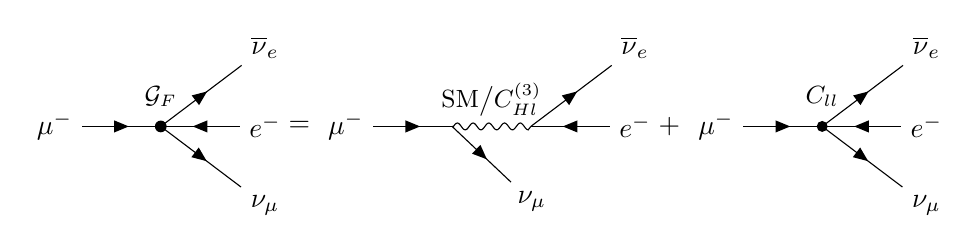
\begin{tikzpicture}
%\tikzset{baseline=(c.base)}
\tikzfeynmanset{inline=(a.base)}
\begin{feynman}
    %diag 1
	\vertex (a);
    \node[circle, fill, inner sep=1.5pt, label={[label distance=0.05cm]90:{\small $\mathcal{G}_F$}}] (circle1) at (a);
    \vertex[right=1cm of a] (f) {$e^-$};
    \vertex[left=1cm of a] (i) {$\mu^-$};
    \vertex[above=1cm of f] (fbar) {$\overline{\nu}_e$};
    \vertex[below=1cm of f] (ibar) {$\nu_\mu$};
    
    \diagram*[baseline=(a.base)] {
      {[edges=fermion]
        (f) -- (a) -- (fbar),
        (i) -- (a) -- (ibar),
      },
    };

    % diag 2
    \vertex[right=3.7cm of a] (b);
    \vertex[right=1cm of b] (b2);
    % \node[circle, fill, label={[label distance=0.05cm]270:{\small SM}] (circleb) at (b);
    \vertex[right=1cm of b2] (f2) {$e^-$};
    \vertex[left=1cm of b] (i2) {$\mu^-$};
    \vertex[above=1cm of f2] (f2bar) {$\overline{\nu}_e$};
    \vertex[below right=1cm of b] (i2bar) {$\nu_\mu$};

    \diagram*[baseline=(b.base)] {
      {[edges=fermion]
        (f2) -- (b2) -- (f2bar),
        (i2) -- (b) -- (i2bar),
      },
      (b) -- [boson, edge label= {\small SM\big/$C_{Hl}^{(3)}$}] (b2)
    };

    %diag 5
    \vertex[right=3.7cm of b2] (e) ;
    \node[circle, fill, inner sep=1.4pt, label={[label distance=0.05cm]90:{\small $C_{ll}$}}] (aux) at (e);
    \vertex[right=1cm of e] (f5) {$e^-$};
    \vertex[left=1cm of e] (i5) {$\mu^-$};
    \vertex[above=1cm of f5] (f5bar) {$\overline{\nu}_e$};
    \vertex[below=1cm of f5] (i5bar) {$\nu_\mu$};

    \diagram*[baseline=(e.base)] {
      {[edges=fermion]
        (f5) -- (e) -- (f5bar),
        (i5) -- (e) -- (i5bar),
      },
    };

    % signs
    \vertex[right=1.5cm of a] (equal) {$=$};
    \vertex[right=1.5cm of b2] (equal) {$+$};

\end{feynman}
\end{tikzpicture} 

\end{document}